\chapter{Analysis}

The analysis encompasses data taken during the 2005 and 2006 RHIC runs when
the polarized proton beams were longitudinally polarized and colliding at a
center-of-mass energy of 200 GeV. Spin asymmetries are constructed using
charged pions produced at mid-rapidity and having large transverse momentum.

\section{$A_{LL}$ Methodology}

We begin with the equation for a double spin asymmetry in terms of directly measurable quantities,
%
\begin{equation}
  A_{LL} = \frac{\sum_{runs} P_{Y}P_{B}\left[(N_{uu} + N_{dd}) - R(N_{ud} + N_{du})\right]}{\sum_{runs} P_{Y}^{2}P_{B}^{2}\left[(N_{uu} + N_{dd}) + R(N_{ud} + N_{du})\right]}.
  \label{eqn:all-basics}
\end{equation}
%
Henceforth parity conservation is employed; the \(++\) subscript denotes a sum
over the \(uu\) and \(dd\) states and the \(+-\) subscript a sum over \(ud\)
and \(du\) states. \(P_Y\) and \(P_B\) are the Yellow and Blue RHIC beam
polarizations, \(N_{ij}\) are spin-dependent charged pion yields, and \(R =
\frac{\mathcal{L}_{++}}{\mathcal{L}_{+-}}\) is a ratio of sampled luminosities
in different spin configurations. Each of the $\mathcal{L}_{ij}$ is a sum of
the scaler counts over bunch crossings with that spin state.

The formula for the statistical uncertainty on \(A_{LL}\) neglects
uncertainties on the relative luminosities and beam polarizations. Assuming
Poisson statistics on \(N_{++}\) and \(N_{+-}\) the uncertainty on the
asymmetry for a single run is
%
\begin{equation}
  \left(\frac{\sigma_{A_{LL}}}{A_{LL}}\right)^2 = \left(N_{++} + R^2 N_{+-}\right)\left[\frac{1}{N^2} + \frac{1}{D^2} - \frac{2 \times COV(N,D)}{ND} \right]
\end{equation}
%
where \(N\) and \(D\) are the numerator and denominator of the raw asymmetry
(that is, neglecting polarizations), and \(COV(N,D) = N_{++} - R^2 N_{+-}\).
In the case of small asymmetries \(\frac{1}{N^2} \gg (\frac{1}{D^2} - \frac{2
COV(N,D)}{ND}\)), and the uncertainty on the numerator dominates the uncertainty
on \(A_{LL}\):
%
\begin{equation}
  \left(\frac{\sigma_{A_{LL}}}{A_{LL}}\right)^2 \approx \frac{N_{++} + R^2 N_{+-}}{N^2}
\end{equation}
%
ROOT's TH1::Divide method does the error propagation correctly in this limit
(it ignores the covariance term). The generalization to a sum over runs is
straightforward since the yields for each run are uncorrelated.

\subsection{Multi-Particle Statistics}

This analysis often accepts multiple pions from a single event. Treating each
of the particles as an independent event and na\"ively using
$\sqrt{N_{pions}}$ for the statistical uncertainty as in the previous section
is not correct. Following the prescription in
\cite{sowinski-multiparticle-statistics} each bin in a histogram is
incremented at most once per event, using a weight equal to the number of
particles that fell into the bin. This technique neglects intra-event particle
correlations across histogram bins.

\subsection{Background Subtraction}

As discussed in Section \ref{sec:pid}, a particle's energy loss per unit path
length (dE/dx) in the TPC provides an effective means of identification across
a broad range of momenta. In the momentum range of interest (2.0 GeV/c and up)
charged pions are not fully separated from heavier charged hadrons (primarily protons and kaons, which have a smaller \(\langle dE/dx \rangle\)) and
electrons (which have a larger \(\langle dE/dx \rangle\)). This contamination is addressed by subtracting the asymmetry of
the background from the raw asymmetry calculated using all
particles in the charged pion acceptance window. The background sidebands located on both sides of the acceptance window have different physical sources and potentially different double spin asymmetries.  The subtraction
procedure must also account for the lack of a clean background sample; the
sidebands themselves have a non-negligible contamination from the charged pion
signal. We start by defining a reduced background fraction to account for the
impurities in the sideband:

\begin{equation*}
  f_{x}(y) = \frac{x~\mathrm{counts~in}~y~\mathrm{window}}{\mathrm{total~ in}~y~\mathrm{window}}
\end{equation*}

\begin{equation*}
  f'(x) = \frac{f_{x}(\pi)}{1 - f_{\pi}(x)}
\end{equation*}
%
The standard equations for the background-subtracted $A_{LL}^{\pi}$ and its
statistical uncertainty are only modified by replacing the background fraction
for each sideband with its reduced background fraction:

\begin{equation}
  A_{LL}^{\pi} = \frac{ A_{LL}^{\pi,raw} - f'(p+K)A_{LL}^{p+K,raw} - f'(e)A_{LL}^{e,raw} }{1 - f'(p+K) - f'(e) },
  \label{eqn:all}
\end{equation}

\begin{equation}
  \sigma_{A_{LL}^{\pi}} = \frac{\sqrt{ \sigma_{A_{LL}^{raw}}^{2} + f'(p+K)^{2} * \sigma_{A_{LL}^{p+K,raw}}^{2} + f'(e)^{2} * \sigma_{A_{LL}^{e,raw}}^{2} }}{1 - f'(p+K) - f'(e)}.
  \label{eqn:sigma-all}
\end{equation}
%
These equations are the final formulae used to calculate the asymmetries for a single STAR run in this work.  The \(raw\) superscript in the formulae denotes an \(A_{LL}\) calculated without background subtraction but taking multi-particle statistics into account.

Equation \ref{eqn:all-basics} specified beam polarizations, spin-dependent relative luminosities, and spin-sorted particle yields as the three components to a double spin asymmetry measurement.  A discussion of the extraction of each of these quantities follows.
\section{Beam Polarizations}

Time-dependent relative beam polarizations are obtained from the pC CNI
polarimeter and normalized by the H-jet polarimeter. pC measurements are made
every few hours during a fill, while the H-jet polarimeter is taking data
almost continuously.

During the 2005 RHIC run pC measurements were generally performed with
vertical targets at one location in \(x\), the horizontal coordinate in the
plane transverse to the beams. The intent was that the measurement be made at
the intensity peak. A small number of explicit polarization profile
measurements were also performed. A study of the normalized event rates
obtained by the polarimeter indicated that the target was occasionally
off-center relative to the beam. In the case of the blue beam, the
polarization showed no dependence on normalized event rate, nor any explicit
dependence on \(x\) in the profile measurements. In contrast, the yellow beam
polarization exhibited a significant normalized rate dependence as well as an
\(x\) dependence in the profile measurements. In the 2006 RHIC run scanning
profile measurements in \(x\) were executed for both beams as the normal mode
of operation as a result of this discovery.

The existence of a non-uniform polarization profile in the beam has
implications for the H-jet normalization procedure. The H-jet target is large
compared to the size of the beam and thus samples the average polarization,
while the pC target is small in one dimension. In order to relate the two one
needs to calculate an average beam polarization from the pC measurements,
which requires knowledge of the beam intensity and polarization profiles in
the transverse dimension orthogonal to the carbon strip. The data from the
2006 polarimeter measurements theoretically enables a direct extraction of
both profiles, but occasional problems with the target positioning render the
procedure somewhat unreliable.

The alternative approach employed by the CNI Polarimeter Group in both the
2005 and 2006 data analyses relies on the assumption that the beam intensity
and polarization profiles are Gaussian with independent widths, and that the
peak of the polarization profile is located at the center of the beam. Then
the polarization \(P\) and normalized event rate \(I\) are related by
%
\begin{equation}
  \frac{P}{P_{max}} = I^R, ~~~~ R=\left(\frac{\sigma_I}{\sigma_P}\right)^2.
  \label{eqn:polarization}
\end{equation}
%
\(P_{max}\) and \(R\) are free parameters determined in a fit to the data (see
Figure \ref{fig:pol_l_lmax}); the average beam polarization in terms of these
parameters is simply
%
\begin{equation}
  \langle P \rangle = \frac{P_{max}}{\sqrt{1+R}}
\end{equation}

\begin{figure}
  \centering
  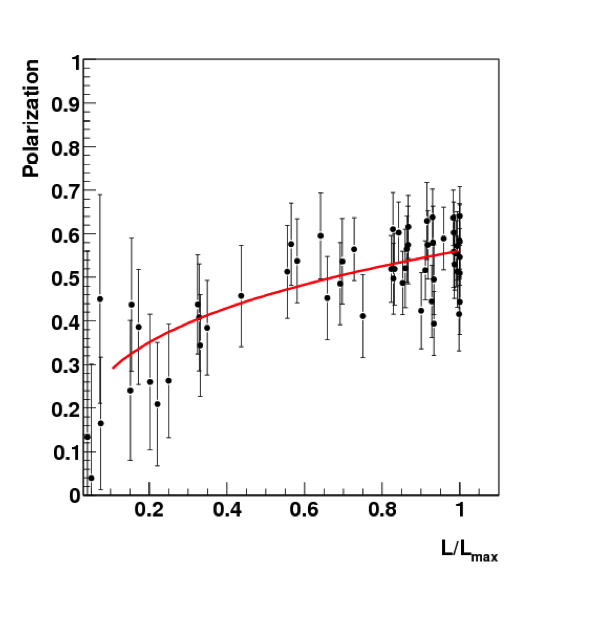
\includegraphics{figures/pol_l_lmax}
  \caption{Example parameterization of beam polarization versus normalized luminosity $I = L/L_{max}$.  The result of the fit is used to calculate the ratio of the widths of the beam intensity and polarization profiles.}
  \label{fig:pol_l_lmax}
\end{figure}

After H-jet normalization, the polarization values reported to the experiments
must be weighted by the product of both beam intensities. Recall that the
value for \(P_{max}\) in \ref{eqn:polarization} already reflects the carbon
ribbon target's uniform cross section in one transverse dimension; the
polarization at the two-dimensional intensity peak is actually
\(P_{max}\sqrt{1+R}\), and the luminosity-weighted average beam polarization
assuming similarly-sized beams (\(\sigma_I^{blue} \approx \sigma_I^{yellow}\))
is then
%
\begin{equation}
  \langle P \rangle_{STAR} = \frac{P_{max} \sqrt{1+R}}{\sqrt{(1+R_x/2)(1+R_y/2)}}.
\end{equation}
%
In the typical pC running mode the carbon ribbon target is vertical, so the
\(R\) in the numerator is more precisely \(R_x\). The polarization profile is
usually much wider than the luminosity profile, so a binomial expansion leads
to
%
\begin{equation}
  \langle P \rangle_{STAR} = P_{max} \sqrt{\frac{1+R_x/2}{1+R_y/2}},
\end{equation}
and in the case where the polarization profiles are similar in both beams, the
luminosity-weighting correction term vanishes. Polarization profile
measurements in the vertical direction are statistically limited in both the
2005 and 2006 datasets but do not indicate any significant difference between
the horizontal and vertical polarization profiles. As a result, the analysis
sets the luminosity-weighting correction term to unity and includes a
systematic uncertainty term reflecting a possible difference in polarization
profiles in the two transverse dimensions.

\begin{figure}
  \subfloat[][Run 5]{
    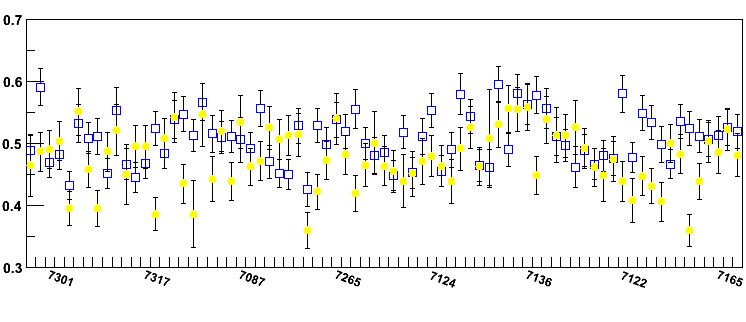
\includegraphics[width=1.0\textwidth]{figures/beam_polarizations_05}
  } \\
  \subfloat[][Run 6]{
    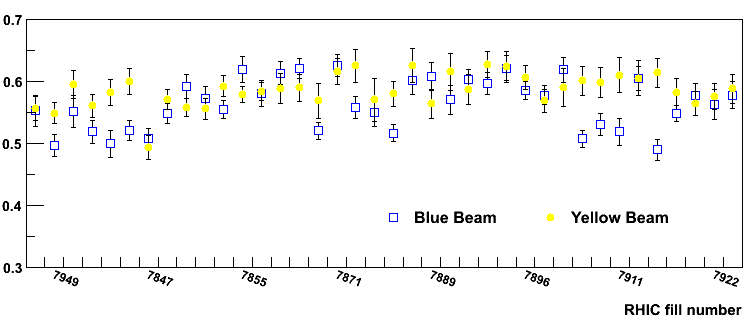
\includegraphics[width=1.0\textwidth]{figures/beam_polarizations_06}
  }
  \caption{RHIC beam polarizations for longitudinally polarized stores analyzed in this work.}
  \label{fig:beam-polarizations}
\end{figure}

The final fill-by-fill beam polarizations are shown in Figure
\ref{fig:beam-polarizations}. The error bars represent statistical and
systematic uncertainties summed in quadrature. The statistical uncertainty for a
fill is obtained by weighting the individual pC measurements in a fill according
to their statistical uncertainty and the duration of time for which the
measurement was ``current''. A variety of sources of systematic uncertainty are
evaluated, including variations in the ``dead layer'' correction that translates
deposited recoil carbon energy to kinetic energy, contributions from molecular
hydrogen in the H-jet target, and imprecise knowledge of the beam polarization
profile. A final tally of the polarizations and their overall uncertainties is
given in Table~\ref{tab:polarizations}. Further details of the analysis can be
found in \cite{CNI05, CNI06}.

\begin{table}
  \centering
  \begin{tabular}{cc|cc}
    \hline
     & & Polarization & Total Uncertainty (dP/P)\\
    \hline
    Run 5 &  Blue & 50.2\% & 5.9\%\\
    Run 5 &  Yellow  & 46.9\% & 6.2\%\\
    Run 5 &  Combined & - & 9.4\%\\
    \hline
    Run 6 &  Blue & 55.9\% & 4.7\%\\
    Run 6 &  Yellow & 58.1\% & 4.8\%\\
    Run 6 &  Combined & - &  8.3\%\\
    \hline
  \end{tabular}
  \caption{Final Beam Polarizations}
  \label{tab:polarizations}
\end{table}

\section{Relative Luminosity Determination}

Bunch-by-bunch beam luminosities are measured using the BBCs and ZDCs and
recorded via the Scaler Boards. The detectors are described in
Sections~\ref{sec:bbc}, \ref{sec:zdc}, and \ref{sec:scalers}. The BBC
measurements are more precise and are employed in the calculation of \(A_{LL}\);
the ZDCs provide a cross-check essential for evaluating systematic
uncertainties.

Various bits of information related to BBC coincidences were encoded on several
Scaler Boards during the 2005 and 2006 RHIC runs. A detailed QA and comparison
of the different boards led to the conclusion that the fine-grained timing
information on boards 5 and 6 should be used to calculate the relative
luminosities. These boards allocated enough bits to track the BBC coincidences
in 16 buckets in \(\Delta T\), the time difference between a hit in the East BBC
and the West BBC. Board 5 was configured to integrate throughout each \(\sim\)
40 minute long STAR run, while board 6 took samples every 250 seconds to allow a
determination of the relative luminosity stability throughout a run.

When possible, the relative luminosities for a run are calculated using the
measurements from board 5. A small number of otherwise-acceptable 2006 runs do
not have reliable scaler information from board 5; in these cases the analysis
relies on the data from board 6. The bunch crossing spin assignments are
obtained using the procedure described in Section \ref{sec:spindb}. The
coincidence count for each bunch crossing is restricted to a set of time buckets
chosen to approximate a 60~cm cut on the $z$ position of the vertex; in the 2005
analysis buckets 7, 8, and 9 are selected, while the 2006 analysis adds bucket 6
into the sum. The relative luminosity \(R\) for a run is then simply the sum of
BBC coincidences in the selected set of time buckets for the bunch crossings
with \(++\) or \(--\) spin assignments divided by the same quantity for bunch
crossings determined to be in a \(+-\) or \(-+\) spin configuration.

% remove runs less than 60 seconds long

% remove runs where the time-integrated BBC coincidence in bit16 < 10k

% remove runs with large number of counts in abort gaps, maybe

% require data from 5/6/11/12, as well as multiple scaler files for the sampling boards

% require that the relative luminosity is fairly stable throughout a fill -- |max(R3) - min(R3)| < 0.0001

% use bit16 on boards 11 and 12, but per-timebin info on boards 5 and 6 (guessing that 11 and 12 don't have timebin info)

% some discrepancies between STAR run stop time and scaler timestamp.  STAR started "getting ahead" of scaler system.  Was anything done about this?  Not clear.  I don't think so

% what was the difference between release 1 and release 2?

\begin{figure}
  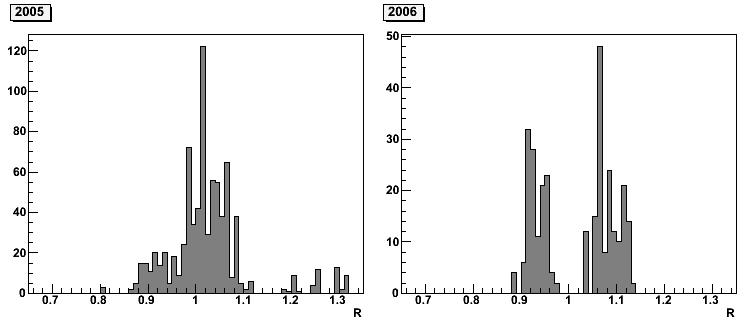
\includegraphics[width=1.0\textwidth]{figures/relative_luminosities}
  \caption{Distributions of per-run values for $R = \frac{\mathcal{L}_{++}}{\mathcal{L}_{+-}}$}
\end{figure}

The statistical uncertainties on $A_{LL}$ assume perfect knowledge of the
relative luminosity of the different spin states. That simplification is
addressed via the systematic uncertainty evaluation described below.

\subsection{Uncertainty Evaluation Using the ZDCs}

% \textit{Note: \href{http://mare.tamu.edu/star/2005n06Jets/2005relLumSys_mar29_2008/}{analysis by Murad Sarsour}}

We can quantify the precision with which we understand the relative luminosities
obtained from the BBCs by using an independent luminosity monitor, the ZDCs. In
the absence of non-statistical fluctuations, the uncertainty on R will be
dominated by the statistics in the ZDCs, which count at a much lower rate than
the BBCs during proton-proton running.

A couple of problems in the ZDC data need to be corrected before a comparison
to the BBCs can be trusted. The first problem is due to the ``killer bit''
algorithm, which suppressed signals in the ZDCs for 10 bunch crossings after
an initial signal. The algorithm is used in heavy ion running to prevent
ringing in the calorimeters from generating false signals, but in pp running
it biases the ZDC counts. Bunch crossings immediately following abort gaps
(where the killer bit is more likely to be off) end up with more ZDC counts
than crossings in the middle of a filled set of bunches. As a result, the
ratio of relative luminosities obtained from the ZDC and BBC will not be flat,
see Figure \ref{fig:zdctobbc6170012zoom}.

\begin{figure}
  \includegraphics[width=1.0\textwidth]{figures/ZDCtoBBC_r7138003}
  \caption{Ratio of uncorrected ZDC and BBC coincidences versus bunch crossing.  The ratio is larger in bunch crossings immediately following abort gaps.}
  \label{fig:zdctobbc6170012zoom}
\end{figure}

The procedure developed to correct for this effect requires scaling the counts
for a given bunch crossing by a factor that takes into account the frequency
with which the previous ten bunch crossings had a signal. For the ZDC singles
rates, the formula for the corrected counts $n_{j}$ in a given bunch crossing
$j$ is
%
\begin{equation}
  n_{j}^{corrected} = n_{j} * \frac{N_{cycles}}{N_{cycles} - \sum_{i=1}^{10}n_{j-i}}
\end{equation}
%
where $N_{cycles}$ is the number of times the beam cycled through STAR in the
run. Figure \ref{fig:zdc-singles-ratio} shows the effect of applying the
correction for a sample run.

\begin{figure}
  \subfloat{
    \includegraphics[width=0.5\textwidth]{figures/ZDCtoBBC_r7133049ER}
  }
  \subfloat{
    \includegraphics[width=0.5\textwidth]{figures/ZDCtoBBC_r7133049WR}
  }
  \caption{Change in the ZDC singles rates after applying the killer bit correction.}
  \label{fig:zdc-singles-ratio}
\end{figure}

The formula to correct the ZDC coincidence counts is complicated by the need to
track the killer bits for the two detectors simultaneously. The formula for the
corrected coincidence counts \(c_{j}^{corrected}\) in a bunch crossing given raw
singles counts \(e_{j}\) (ZCDE) and \(w_{j}\) (ZDCW) and coincidence counts
\(c_{j}\) is
%
\begin{align}
  &\alpha_{j} = N_{cycles} - \sum_{i=1}^{10}c_{j-i} \notag\\
  &\beta_{j} = E_{j-10} + W_{j-10} + E_{j-9}*\left(1 - \frac{W_{j-10}}{\alpha_{j} - E_{j-10}}\right) + W_{j-9}*\left(1 - \frac{E_{j-10}}{\alpha_{j} - W_{j-10}}\right) + ...\notag\\
  &c_{j}^{corrected} = c_{j} * \frac{N_{cycles}}{\alpha_{j} - \beta_{j}} 
\end{align}
%
where \(E(W)_{j-i} \equiv e(w)_{j-i} - c_{j-i}\) is the ZDCE(W) singles count
minus the coincidence count for the j-ith bunch crossing. The effect of the
killer bit correction on the coincidence distributions is shown in Figure
\ref{fig:coinRat6143016}.

\begin{figure}
  \begin{center}
    \includegraphics[width=0.6\textwidth]{figures/ZDCtoBBC_r7133049coin}
  \end{center}
  \caption{Change in the ZDC coincidence rates after applying the killer bit
  correction.}
  \label{fig:coinRat6143016}
\end{figure}

\begin{figure}
  \begin{center}
    \includegraphics[width=0.8\textwidth]{figures/c7308}
  \end{center}
  \caption{Example of a coherent spin pattern and even-odd ZDC rate
  oscillation. In this case, the ZDC rate is always higher when the spin of
  the blue beam is down.}
  \label{fig:c7308}
\end{figure}

% More Details on even-odd effect
% http://cyclotron.tamu.edu/star/2006Jets/jul31_2007/
% http://cyclotron.tamu.edu/star/2006Jets/aug2_2007/ - figure 4 on this page plots the asymmetry between the ZDC/BBC ratio for even bxings and the ZDC/BBC ratio for odd bxings.  The asymmetry can be positive or negative even within a spin pattern, basically no correlation.  But at the bottom of the page, Murad clearly shows that the even/odd asymmetry arises from the ZDCs, not the BBCs, when he plots a particular jet asymmetry using R_ZDC and then R_BBC, and compares the sign of that asymmetry to the sign of the asymmetry in Figure 4.

% the cut on |F*(S-1)| < 0.002 is strictly a 2005 thing, in 2006 the ZDC coincidences are actually renormalized! Uber-sketchy if you ask me.

The second problem in need of correction has come to be known as the
``even-odd'' effect.  The ZDC coincidence rates are often
different for even-numbered and odd-numbered bunch crossings, due to
oscillations in the electronics pedestals in specific ADC channels of the CDB
boards used to read out the ZDCs. This oscillation can introduce a false
asymmetry if it aligns coherently with a particular spin pattern. For instance,
in Figure \ref{fig:c7308} the ZDC coincidence rates are always higher when the
spin of the blue beam is down.  To quantify the bias this introduces on $A_{LL}$, we can
define the fractional overlap between the even-odd ZDC oscillation and relevant
portion of the spin pattern for $A_{LL}$ using a 120 element vector $|EO\rangle
= |+1,-1,+1,-1,...\rangle$ and another 120 element vector $|LL\rangle$ whose
elements are 1 if the bunch crossing is UU or DD, -1 if UD or DU, and 0
otherwise. The inner product of these vectors measures the susceptibility of
$A_{LL}$ for that spin pattern to any even-odd oscillation.

% \begin{figure}
%   \includegraphics[width=1.0\textwidth]{figures/fevfod}
%   \caption{Magnitude of even-odd rate asymmetry versus time in the 2005 RHIC run.}
%   \label{fig:fevfod}
% \end{figure}

It turns out that $A_{LL}$ is less biased by the even-odd rate oscillation in
the ZDC than, say, the blue beam single-spin asymmetry. Figure \ref{fig:cll}
plots the fill-by-fill change in $A_{LL}$ if the ZDC is used for relative
luminosities instead of the BBC against the the product of the fractional
overlap $F \equiv \langle EO | LL \rangle$ and the magnitude of the even-odd
oscillation $S-1$. Placing a cut on $|F*(S-1)| < 0.002$ is well-motivated. For
fills without reliable ZDC information, we use Figure \ref{fig:fevfod} to
assume a conservative $|S-1| = 0.03$.

\begin{figure}
  \begin{center}
  \includegraphics[]{figures/cll}
  \end{center}
  \caption{Change in $A_{LL}$ versus the product of the even-odd rate oscillation amplitude and the fractional overlap $\langle EO | LL \rangle$.  Deviations from 0 on the x-axis indicate fills where $A_{LL}$ is biased by the even-odd effect.}
  \label{fig:cll}
\end{figure}

After correcting for the killer bits and rejecting the fills that fail the
even-odd oscillation cut the ZDC coincidences counts for even and odd bunch
crossings are separately normalized using the following normalization factors:
%
\begin{equation}
  f_{even} = \frac{\langle ZDC/BBC \rangle}{\langle ZDC_{even}/BBC_{even} \rangle}, ~~~~
  f_{odd} = \frac{\langle ZDC/BBC \rangle}{\langle ZDC_{odd}/BBC_{odd} \rangle};
\end{equation}
%
that is, the ZDC coincidence counts for even(odd)-numbered bunch crossings in a
run are rescaled by the mean ZDC/BBC ratio for the run divided by the mean
ZDC/BBC ratio for even(odd)-numbered bunch crossings in the run. Finally, the
uncertainty on $A_{LL}$ due to the uncertainty in the relative luminosities is
calculated as the change in \(A_{LL}\) when the relative luminosities are
supplied by the normalized ZDCs instead of the BBCs, and is equal to
$9.4\times10^{-4}$.

% \subsection{Beam Background Bias}
% 
% % \textit{Note: \href{http://www.star.bnl.gov/protected/spin/kowalik/2005/r-lumi/bkg_sys.html}{analysis by Kasia Kowalik}}
% 
% The relative luminosities obtained from the BBCs might also be biased by false
% signals generated by beam-gas background. We can try to quantify this by
% studying the coincidence rate in crossings where one of the two beams has an
% unfilled bunch (``abort gaps''). The beam-gas background is assumed to be
% crossing- and spin-independent, but it can be different in each beam. It follows
% that the per-crossing coincidence rate due to beam-gas in each beam is just the
% average number of BBC coincidences found in the abort gaps for that beam. In
% Figure \ref{fig:bkg-yellow-blue}, the x-axis is the background rate divided by
% the total rate, defined as the average number of coincidences per bunch crossing
% with a spin state of \(++\), \(+-\), \(-+\), or \(--\). The two histograms are
% incremented for each STAR run. We see that the background rate in the BBCs due
% to beam-gas is typically less than 0.1\% of the total rate.
% 
% \begin{figure}
%   \includegraphics[width=1.0\textwidth]{figures/bkg-yellow-blue}
%   \caption{Fraction of the total coincidence rate attributed to beam gas in
%   each beam. The histograms are incremented once for each STAR run.}
%   \label{fig:bkg-yellow-blue}
% \end{figure}
% 
% Given run-dependent background fractions for both beams, it's possible to
% calculate background-subtracted relative luminosities. Figure
% \ref{fig:r-lumi-sys-bkg} shows the difference between the raw relative
% luminosity and the background-subtracted version. The background-corrected
% relative luminosities yield an $A_{LL}$ that differs from the original by
% $3.0\times10^{-4}$, so we use that as the uncertainty for this source of
% systematic error.
% 
% \begin{figure}
%   \begin{center}
%     \includegraphics[width=0.6\textwidth]{figures/r-lumi-sys-bkg}
%   \end{center}
%   \caption{Change in the relative luminosities after correcting for beam-gas
%   background.}
%   \label{fig:r-lumi-sys-bkg}
% \end{figure}

\section{Spin-Sorted Yields}

\subsection{Run and Event Selection}

% total number of runs containing triggered events

% -- so many runs get tossed out, though

% describe QA checks
% - use the best reconstructed vertex for the event.  If no vertex was reconstructed, skip the event
% - identified spin states for the colliding bunches in both beams
% - vertex position from scaler timing information falls within a window

% list numbers of runs that survive those checks, as well as corresponding sampled luminosity

\subsection{Pion Identification}

Charged pions are identified from the subset of primary tracks in each event
having at least 25 fit points, a distance of closest approach (DCA) to the
primary vertex of no more than 1 centimeter, a pseudorapidity magnitude less
than 1.0, and a transverse momentum greater than 2.0 GeV/c. The first three cuts
select high quality tracks. The transverse momentum cut is not necessary from an
experimental perspective, but an \(A_{LL}\) analysis of low momentum pions
offers limited physics insights and the analysis can proceed more efficiently if
these very common particles are not included. The determination of the PID
acceptance window is discussed in Section~\ref{sec:pid} and the window
boundaries are listed in Table~\ref{tbl:pid-selection-windows}.
Figure~\ref{fig:pid-accept-window} highlights the characteristic MIP
distribution of the accepted charged pion tracks.

% TODO drift velocity fix?  cool to include, since I did it. Not needed though

\begin{table}
  \centering
  \begin{tabular}{|c|c|}
    \hline
    Criterion & Efficiency \\
    \hline
    $|\eta| < 1.0$ & 0.94 \\
    at least 25 fit points & 0.95 \\
    $|DCA|$ of associated global track $<$ 1.0 cm & 0.96 \\
    \hline
  \end{tabular}
  \caption{Quality cuts imposed on the high-$p_T$ primary tracks before PID selection.}
\end{table}

\begin{figure}
  \centering
  \includegraphics[width=0.5\textwidth]{figures/placeholder}
  \caption{Energy loss per unit path length versus momentum for tracks produced by identified charged pions.}
  \label{fig:pid-accept-window}
\end{figure}

\subsection{Jet-Pion Correlations}

% TODO description of QA procedure? (essentially jet QA)

In the 2006 data analysis events are accepted only if they contain a
reconstructed jet with an uncorrected \(p_T\) between 10 and 30 GeV/c, a
pseudorapidity between -0.7 and 0.9, and an electromagnetic energy fraction not
greater than 0.92. Furthermore, the difference in azimuth between the jet axis
and the center of a jet patch above the trigger threshold must be no more than
\(36^\circ\). Multiple jets in an event can satisfy these ``trigger jet'' cuts.

Charged pions satisfying the track quality and PID cuts described in the
preceding section are compared against the list of trigger jets. If a charged
pion is separated from a trigger jet by at least 2.0 radians in azimuth it is
considered to be an ``away-side'' pion and is accepted for analysis.
Figure~\ref{fig:dphi} plots the azimuthal distribution of charged pions relative
to trigger jets in the 2006 analysis. The data show good agreement with Monte
Carlo simulations.

\begin{figure}
  \centering
  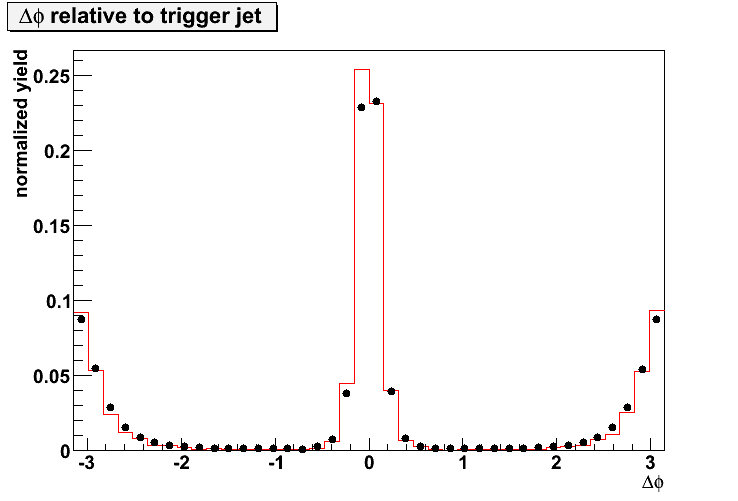
\includegraphics[width=0.7\textwidth]{figures/dphi}
  \caption{Azimuthal distribution of charged pions relative to the trigger jet axis in the 2006 dataset.  The black circles represent data, the red lines fully reconstructed Monte Carlo. Pions with $|\Delta \phi| > 2.0$ are accepted for analysis.}
  \label{fig:dphi}
\end{figure}

The data are binned as a function of \(z\), defined as the ratio of the
away-side pion \(p_T\) and the trigger jet \(p_T\). Figure~\ref{fig:meanpt}
shows that the jet \(\langle p_T \rangle\) is approximately constant as a
function of \(z\), and thus that the charged pion \(\langle p_T \rangle\)
increases linearly with \(z\). Again, the data are modeled well by STAR's
Pythia+GEANT simulations.

\begin{figure}
  \centering
  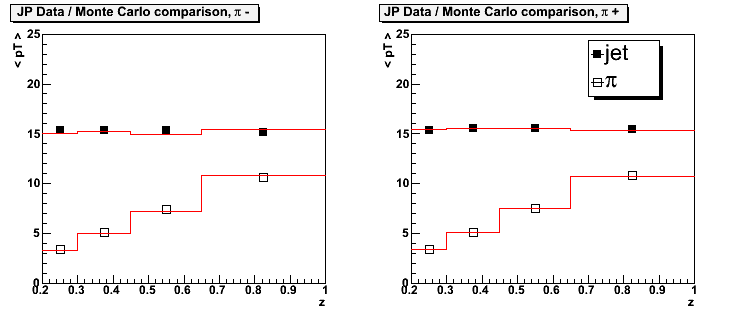
\includegraphics[width=1.0\textwidth]{figures/meanpt}
  \caption{Comparison of the $\langle p_T \rangle$ values for jets and charged pions in each $z$ bin.  The data show good agreement with fully reconstructed Pythia+GEANT events that pass a simulation of the BJP2 trigger.}
  \label{fig:meanpt}
\end{figure}

\section{Systematic Uncertainty Evaluations}
% beam polarization vectors and A_sigma - 1 day.  Don't go into too many details of the determination of the beam vector, just say it was based on an analysis of left/right and up/down asymmetries in the BBCs during longitudinal and transverse running.

\subsection{Polarization Vectors and Transverse Asymmetries}

The BBCs enable local polarimetry at STAR.  Vertical polarization in the beam generates an asymmetry in the counts recorded by the left and right halves of the BBC on which it impinges, while radial polarization generates an asymmetry in the top and bottom halves of the detector.  An accurate accounting of residual non-longitudinal polarization in the beams is important, because a double transverse spin asymmetry \(A_{\Sigma}\) could generate a false \(A_{LL}\).  The size of this false signal is given by the equation
%
\begin{equation}
  \delta A_{LL}^{\mathrm{non-longitudinal}} = | \tan(\theta_B) \tan(\theta_Y) \cos(\phi_B - \phi_Y) A_{\Sigma} |.
  \label{eqn:pol-vector-uncertainty}
\end{equation}
%
The beam polarization angles at STAR are determined through an analysis of cross ratios in the BBCs \cite{Kiryluk:2005gg}.  These ratios are directly sensitive to the azimuthal angle of the beam, and a comparison of the ratios in longitudinal and transverse running allows an extraction of the angle of inclination.  The measured ratio is 
%
\begin{equation}
  \epsilon_{BBC} = \frac{r_{ij} -1}{r_{ij} + 1} \simeq \left\{
  \begin{array}{l l}
    A_N^{BBC} \times P_v \times \langle \cos \phi \rangle & i,j = \mbox{Left, Right} \\
    A_N^{BBC} \times P_r \times \langle \sin \phi \rangle & i,j = \mbox{Up, Down} \\
  \end{array} \right.
\end{equation}
%
in which \(r_{ij} = \sqrt{\frac{N_i^{\uparrow} N_j^{\downarrow}}{N_i^{\downarrow} N_j^{\uparrow}}}\) and \(N_{i(j)}^{\uparrow(\downarrow)}\) are the spin dependent yields on the Left(Right) or Up(Down) side of the detector. \(P_{v(r)}\) is the vertical (radial) beam polarization.  Table~\ref{tab:pol-vectors} tabulates the extracted polarization vectors from measurements of the BBC cross-ratios.  There are two separate extractions for the 2006 data because the spin rotator magnets were adjusted midway through the run.  The data show a steady improvement in the performance of the spin rotators.

% due to the large non-statistical variations, ∼1.5 degrees, in the estimate of the polar angle coming from the the up/down asymmetries in the transverse running, we decided to use a conservative estimate of cos(φY − φB) = 1.

% that doesn't make much sense ... UD transverse asymmetries don't contribute to the determination of the polar angle to first order.

% also, the formulae to get the beam angles from these asymmetries are inconsistent.  But Murad's numbers for tan(theta) and phi do yield his numbers for the multiplicative factor in front of Asigma

% Table of Beam Polarization Vectors
\begin{table}
  \begin{center}
    \begin{tabular}{l|c|c}
      Run Period & Blue ($\theta, \phi$) & Yellow ($\theta, \phi$) \\
      \hline
      2005 & (7.9, 74.0) & (17.2, 138.7) \\
      2006a (7132001-7138034) & (6.9, 87.7) & (10.0, 34.4) \\ 
      2006b (7138035-7156040) & (0.9, 69.3) & (3.9, -47.8)
    \end{tabular}
  \end{center}
  \caption{Beam polarization vectors as determined from an analysis of up-down and left-right asymmetries in the BBCs.  The spin rotators were adjusted midway through the second longitudinal running period in 2006.}
  \label{tab:pol-vectors}
\end{table}


% use cos(phi_B - phi_Y) = 1 as conservative estimate since polar angle measurements exhibit non-statistical fluctuations in 2006.

% asigma graphs for 2006, cleaned up

% limited transverse running in 2005, different trigger thresholds in 2006.  Not fair to calculate A_sigma in 2006 and use it for 2005.  Assume 10%, flat in pT.  Not sure if it's justified by any data analysis I've done.


\subsection{Trigger Bias}

STAR's BEMC jet patch trigger preferentially selects events where one of the
jets is located at mid-rapidity and hadronizes with a strong electromagnetic
component. This preference indirectly biases the triggered sample toward events
containing a quark jet, since quark jets have a harder fragmentation profile
than gluon jets. In addition, the jet that fires the trigger is unlikely to
contain a leading charged pion. The fragmentation bias in the trigger jet is a
primary reason that our analysis of the 2006 data is restricted to pions
opposite the trigger jet in azimuth.

The various biases introduced by the trigger are evaluated using a leading-order
Monte Carlo simulation of \(A_{LL}\) known as the Method of Asymmetry Weights.
Pythia supplies the kinematics and hard scattering subprocess of each simulated
event, which are sufficient to determine the partonic \(a_{LL}\) (calculated at
NLO in \cite{}). An ``asymmetry weight'' for the event is then constructed by
statistically sampling parton distribution functions:
%
\begin{equation}
  w = \frac{\Delta f_1(x_1, Q^2) * \Delta f_2(x_2, Q^2) * a_{LL}}{f_1(x_1, Q^2) * f_2(x_2, Q^2)},
\end{equation}
%
and one arrives at a Monte Carlo \(A_{LL}\) by simply taking the ratio of
asymmetry-weighted and unweighted distributions. The difference between the
\(A_{LL}\) for all Pythia events and the \(A_{LL}\) for reconstructed events
that satisfy a simulated trigger condition is used to assign the systematic
uncertainty.

\subsubsection{Monte Carlo Fragmentation Modeling}

The procedure described above requires that the Monte Carlo generator accurately
reproduces the real event kinematics. Unfortunately, the fragmentation tune in
Pythia~6 is not quite up to the task for STAR.
Figure~\ref{fig:subprocess-fractions} is a comparison of the subprocess
contributions to charged pion production reported by Pythia with the results of
NLO pQCD calculations incorporating Kretzer and DSS fragmentation functions. The
DSS set is known to better describe RHIC kinematics, but in
Figure~\ref{fig:subprocess-fractions} it's clear that Pythia agrees much better
with the Kretzer set.

\begin{figure}
  \subfloat[Kretzer]{
    \includegraphics[width=0.5\textwidth]{figures/pythia-kretzer}
    \label{fig:pythia-kretzer}
  }
  \subfloat[DSS]{
    \includegraphics[width=0.5\textwidth]{figures/pythia-dss}
    \label{fig:pythia-dss}
  }
  \caption{Comparison of subprocess contributions to charged pion production
  in Pythia and NLO pQCD calculations incorporating two different
  fragmentation functions.  The data points are results from Pythia and are the same in both plots. The Pythia results agree much better with the
  calculations using Kretzer fragmentation functions}
  \label{fig:subprocess-fractions}
\end{figure}

An accurate simulation of the subprocess contributions is an important
precondition for using the Method of Asymmetry Weights to evaluate trigger and
reconstruction bias, quite simply because $A_{LL}$ has such a strong subprocess
dependence. To confirm that the problem is really isolated to Pythia's
fragmentation functions, we examined the ratio of pions fragmenting from the
quark and the gluon in \(qg\) scattering events. That ratio is shown in Figure
\ref{fig:qg-fragmentation}, and confirms that the fragmentation model is
Kretzer-like, with much softer gluon fragmentation and/or harder quark
fragmentation than is observed at RHIC.

\begin{figure}
  \begin{center}
    \includegraphics[width=0.7\textwidth]{figures/qg-fragmentation}
  \end{center}
  \caption{Fraction of pions produced in quark-gluon scattering events that
  fragment from the gluon. Once again, the Pythia distributions agree much
  better with the calculation that uses Kretzer fragmentation functions.}
  \label{fig:qg-fragmentation}
\end{figure}

% the reweighting factor is the ratio of DSS and Kretzer FFs in each pT bin

% this reweighting factor is not applied in the 2006 analysis at the moment

Rather than plumb the depths of Pythia's independent fragmentation model, this
analysis applied a $p_{T}$- and subprocess-dependent reweighting factor to the
simulations to generate DSS-like fragmentation. The effect of this reweighting
is shown in Figure \ref{fig:compare-mcasym-nlo}. The filled markers show
markedly better agreement with the NLO pQCD calculations than the open markers,
particularly in scenarios such as GRSV-MIN where the difference in $A_{LL}$
between \(gg\) and \(qg\) subprocesses is large. The agreement is still not
perfect; one might speculate that Pythia gives too much weight to favored quark
fragmentation, since at high $p_{T}$ the $\pi^{-}$ asymmetries are too small
(indicating a relatively large d quark contribution) and the $\pi^{+}$
asymmetries are too large (consistent with a large u quark contribution).
However, as the trigger and reconstruction are not expected to be quark flavor
dependent we have decided to press forward with these simulations.

\subsubsection{2005 Bias Calculations}

\begin{figure}
  \includegraphics[width=\textwidth]{figures/compare-mcasym-nlo}
  \caption{Comparison of Monte Carlo asymmetries with NLO pQCD calculations
  incorporating DSS fragmentation functions. The open markers show results
  obtained using STAR's Pythia tune. The filled markers show the change in the
  asymmetries after reweighting the gg, qg, and qq distributions by the ratio
  of subprocess fractions calculated using DSS and Kretzer fragmentation
  functions.}
  \label{fig:compare-mcasym-nlo}
\end{figure}

Figure \ref{fig:mcasym-diff} examines the difference between asymmetries for a
``true'' sample using untriggered events and pions pulled straight from the
Pythia record, and a ``trigger+reco'' sample where the events must satisfy the
JP2 trigger simulator and the pion kinematics are obtained from TPC track
reconstruction. In some cases, the difference between the two samples is smaller
than the uncertainty on the ``trigger+reco'' sample (see Figure
\ref{fig:mcasym-sigma}). The systematic is assigned as the larger of the
difference in central values and the uncertainty on the ``trigger+reco'' sample.

The size of the systematic obviously depends on the polarized gluon
distributions that are included in the analysis. Previous measurements have
excluded the maximal polarization scenarios as well as scenarios with the
functional form of the GRSV set and integral gluon polarizations larger than 0.3
at \(Q^2 = 1 GeV^2\). As a result, we use an envelope defined by the GRSV M030
and P030 scenarios. The results of this analysis for the 2005 dataset are shown
in Table \ref{tbl:trig-reco-bias}.

% TODO recalculate bias systematic using M030 - P030 scenarios
% TODO better-looking plots for asymmetry difference and uncertainty

\begin{figure}
  \includegraphics[width=\textwidth]{figures/mcasym_run5_diff_rescaled}
  \caption{Difference between true and reconstructed Monte Carlo
  asymmetries after fragmentation reweighting.  The cyan and magenta curves represent polarized gluon distributions with the functional form of GRSV STD but with varying integral values for $\Delta G$.}
  \label{fig:mcasym-diff}
\end{figure}

\begin{figure}
  \includegraphics[width=\textwidth]{figures/mcasym_run5_sigma_rescaled}
  \caption{Uncertainty on reconstructed Monte Carlo asymmetries. If the
  uncertainty is larger than the difference between true and reconstructed
  asymmetries we use this to assign the systematic instead.}
  \label{fig:mcasym-sigma}
\end{figure}

\begin{table}[ht]
    \begin{center}
        \begin{tabular}{c|c|c}
        \hline
        $p_{T}$ & $\pi^{-}$ $\delta A_{LL}$ & $\pi^{+}$ $\delta A_{LL}$\\
        \hline
        2.00 - 3.18 & -0.0059 +0.0027 & -0.0061 +0.0061\\
        3.18 - 4.56 & -0.0083 +0.0072 & -0.0128 +0.0066\\
        4.56 - 6.32 & -0.0093 +0.0034 & -0.0176 +0.0101\\
        6.32 - 8.80 & -0.0072 +0.0036 & -0.0209 +0.0186\\
        8.80 - 12.84 & -0.0048 +0.0057 & -0.0152 +0.0062\\
    \hline
    \end{tabular}
    \end{center}
    \caption{2005 Trigger and Reconstruction Bias Uncertainties}
    \label{tbl:trig-reco-bias}
\end{table}

\subsubsection{2006 Bias Calculations}

An additional complication for the 2006 data analysis is shown in
Figure~\ref{fig:mean-pt-simu}. The JP trigger efficiency is a sharply-rising
function of jet \(p_T\); as a result, the \(\langle p_T \rangle\) for pions and
especially for jets in a given \(z\) bin is significantly larger in the
triggered sample compared to the minimum-bias sample. In effect, we are
under-sampling the low \(x\) regime in each \(z\) bin. The bias calculated by a
na\"ive application of the Method of Asymmetry Weights to this measurement would
be unacceptably large. Instead, we choose to publish the trigger efficiency as
part of the measurement, and to rescale the minimum-bias Monte Carlo sample by
that trigger efficiency. A comparison of the simulated \(A_{LL}\) in the
triggered and rescaled minimum-bias samples allows an estimate of the
measurement error introduced by the trigger's subprocess bias.

\begin{figure}
  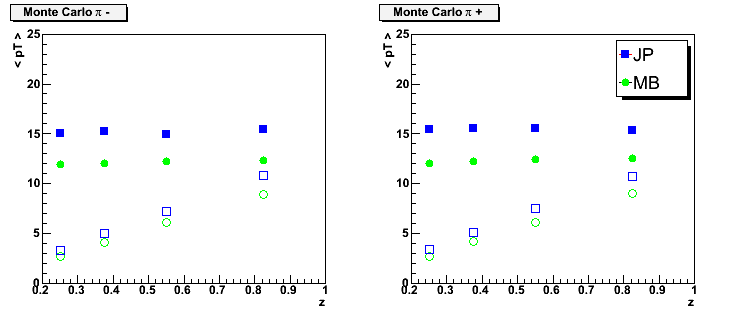
\includegraphics[width=1.0\textwidth]{figures/meanpt-by-trigger}
  \caption{Comparison of the $\langle p_T \rangle$ for MB and JP triggers ni the 2006 Monte Carlo.  Filled markers plot jet $\langle p_T \rangle$ and open markers charged pion $\langle p_T \rangle$. The JP triggered data sample has a dramatically larger jet $\langle p_T \rangle$ in each $z$ bin, which biases $A_{LL}$ towards larger values in the GRSV framework.}
  \label{fig:mean-pt-simu}
\end{figure}

Figure~\ref{fig:trigger-efficiency} plots the ratio of jet yields in the MB
Monte Carlo sample and the sample that passes a simulated JP trigger. The
trigger efficiency as a function of jet \(p_T\) is well described by a cubic
polynomial:
%
\begin{equation}
  \epsilon_{trigger} = 1.149 - 0.2655 * p_T   + 0.01857 * p_T^2 - 0.0003445 * p_T^3.
  \label{eqn:trigger-efficiency}
\end{equation}
%
Finally, Figure~\ref{fig:trig-bias-2006} plots the difference between the
trigger sample \(A_{LL}\) and the \(A_{LL}\) calculated from the rescaled MB
sample for an envelope of GRSV parameterizations with integral gluon
polarization less than 0.3 at \(Q^2 = 1 GeV^2\). A systematic uncertainty on our
measured \(A_{LL}\) is assigned by taking the maximum asymmetry difference in
each bin, or the uncertainty on the triggered \(A_{LL}\) if all asymmetry
differences are consistent with zero. The final values are tabulated in
Table~\ref{tab:trig-bias-2006}.

% TODO 2006 mcasym numbers for M030-P030
% TODO reweight 2006 Monte Carlo by DSS/Kretzer ratio

\begin{figure}
  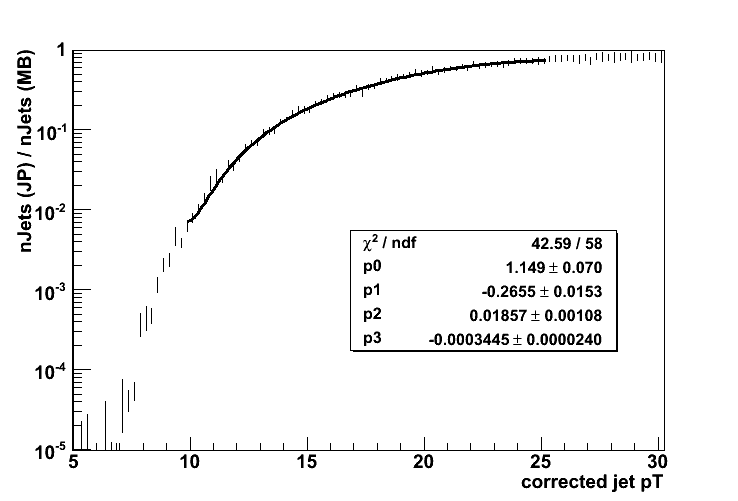
\includegraphics[width=1.0\textwidth]{figures/trigger-efficiency}
  \caption{A parameterization of the BJP1 trigger efficiency as a function of corrected jet $p_T$ established from the 2006 Monte Carlo.  This parameterization is used to factor out the trigger efficiency from the Method of Asymmetry Weights $A_{LL}$ studies, allowing those studies to focus on the subprocess bias inherent in the trigger.}
  \label{fig:trigger-efficiency}
\end{figure}

\begin{figure}
  \centering
  \includegraphics[width=0.5\textwidth]{figures/placeholder}
  \caption{Comparison of simulated asymmetries for triggered events and minimum-bias events which have been rescaled to reflect the average trigger efficiency as a function of jet $p_T$. The resulting difference is a measure of the bias introduced by the subprocess-dependence in the trigger.}
  \label{fig:trig-bias-2006}
\end{figure}

\begin{table}[ht]
    \begin{center}
        \begin{tabular}{c|c|c}
        \hline
        $z$ & $\pi^{-}$ $\delta A_{LL}$ & $\pi^{+}$ $\delta A_{LL}$\\
        \hline
        0.20 - 0.30 & 0.0 &  0.0 \\
        0.30 - 0.45 & 0.0 &  0.0 \\
        0.45 - 0.65 & 0.0 &  0.0 \\
        0.65 - 1.00 & 0.0 &  0.0 \\
    \hline
    \end{tabular}
    \end{center}
    \caption{2006 Trigger and Reconstruction Bias Uncertainties}
    \label{tab:trig-bias-2006}
\end{table}



% \subsection{Polarization Vectors and Transverse Asymmetries}

% data selection - 1/2 day

% pion identification - 1 day

% jet reconstruction - 1 day

% jet/pion correlations - 1/2 day.  Just a plot of the dphi matching in data and simulation ought to be enough.

% Systematic Uncertanties

% nothing for PID, but will i need to redo the run 6 analysis to subtract backgrounds? yes.  Can I assume nSigmaPion does not need to be recalibrated? probably - 4 days

% 2006 trigger bias includes the minbias Monte Carlo reweighting hackery - 2 days

% but not just the reweighting hackery, there's also an uncertainty in the size of the jet pT shift - 1 day.  And why don't I include pion pt shifts in that calculation?  Is it because I choose bin widths to match the pion pT resolution?

% Results - 1 day

% Conclusions - 1.5 days

% Cleanup - 2 days
